\documentclass[A4paper,12pt]{article}

% Этот шаблон документа разработан в 2014 году
% Данилом Фёдоровых (danil@fedorovykh.ru) 
% для использования в курсе 
% <<Документы и презентации в \LaTeX>>, записанном НИУ ВШЭ
% для Coursera.org: http://coursera.org/course/latex .
% Исходная версия шаблона --- 
% https://www.writelatex.com/coursera/latex/5.3

% В этом документе преамбула

%%% Работа с русским языком
\usepackage{cmap}					% поиск в PDF
\usepackage{mathtext} 				% русские буквы в формулах
\usepackage[T2A]{fontenc}			% кодировка
\usepackage[utf8]{inputenc}			% кодировка исходного текста
\usepackage[english,russian]{babel}	% локализация и переносы
\usepackage{indentfirst}
\frenchspacing

\renewcommand{\epsilon}{\ensuremath{\varepsilon}}
\renewcommand{\phi}{\ensuremath{\varphi}}
\renewcommand{\kappa}{\ensuremath{\varkappa}}
\renewcommand{\le}{\ensuremath{\leqslant}}
\renewcommand{\leq}{\ensuremath{\leqslant}}
\renewcommand{\ge}{\ensuremath{\geqslant}}
\renewcommand{\geq}{\ensuremath{\geqslant}}
\renewcommand{\emptyset}{\varnothing}

%%% Дополнительная работа с математикой
\usepackage{amsmath,amsfonts,amssymb,amsthm,mathtools} % AMS
\usepackage{icomma} % "Умная" запятая: $0,2$ --- число, $0, 2$ --- перечисление

%% Номера формул
%\mathtoolsset{showonlyrefs=true} % Показывать номера только у тех формул, на которые есть \eqref{} в тексте.
%\usepackage{leqno} % Нумереация формул слева

%% Свои команды
\DeclareMathOperator{\sgn}{\mathop{sgn}}

%% Перенос знаков в формулах (по Львовскому)
\newcommand*{\hm}[1]{#1\nobreak\discretionary{}
	{\hbox{$\mathsurround=0pt #1$}}{}}

%%% Работа с картинками
\usepackage{graphicx}  % Для вставки рисунков
\graphicspath{{images/}{images2/}}  % папки с картинками
\setlength\fboxsep{3pt} % Отступ рамки \fbox{} от рисунка
\setlength\fboxrule{1pt} % Толщина линий рамки \fbox{}
\usepackage{wrapfig} % Обтекание рисунков текстом

%%% Работа с таблицами
\usepackage{array,tabularx,tabulary,booktabs} % Дополнительная работа с таблицами
\usepackage{longtable}  % Длинные таблицы
\usepackage{multirow} % Слияние строк в таблице

%%% Теоремы
\theoremstyle{plain} % Это стиль по умолчанию, его можно не переопределять.
\newtheorem{theorem}{Теорема}[section]
\newtheorem{proposition}[theorem]{Утверждение}

\theoremstyle{definition} % "Определение"
\newtheorem{corollary}{Следствие}[theorem]
\newtheorem{problem}{Задача}[section]

\theoremstyle{remark} % "Примечание"
\newtheorem*{nonum}{Решение}

%%% Программирование
\usepackage{etoolbox} % логические операторы

%%% Страница
\usepackage{extsizes} % Возможность сделать 14-й шрифт
\usepackage{geometry} % Простой способ задавать поля
\geometry{top=30mm}
\geometry{bottom=40mm}
\geometry{left=30mm}
\geometry{right=20mm}
%
%\usepackage{fancyhdr} % Колонтитулы
% 	\pagestyle{fancy}
%\renewcommand{\headrulewidth}{0pt}  % Толщина линейки, отчеркивающей верхний колонтитул
% 	\lfoot{Нижний левый}
% 	\rfoot{Нижний правый}
% 	\rhead{Верхний правый}
% 	\chead{Верхний в центре}
% 	\lhead{Верхний левый}
%	\cfoot{Нижний в центре} % По умолчанию здесь номер страницы

\usepackage{setspace} % Интерлиньяж
\onehalfspacing % Интерлиньяж 1.5
%\doublespacing % Интерлиньяж 2
%\singlespacing % Интерлиньяж 1

\usepackage{lastpage} % Узнать, сколько всего страниц в документе.

\usepackage{soul} % Модификаторы начертания

\usepackage{hyperref}
\usepackage[usenames,dvipsnames,svgnames,table,rgb]{xcolor}
\hypersetup{				% Гиперссылки
	unicode=true,           % русские буквы в раздела PDF
	pdftitle={Заголовок},   % Заголовок
	pdfauthor={Автор},      % Автор
	pdfsubject={Тема},      % Тема
	pdfcreator={Создатель}, % Создатель
	pdfproducer={Производитель}, % Производитель
	pdfkeywords={keyword1} {key2} {key3}, % Ключевые слова
	colorlinks=true,       	% false: ссылки в рамках; true: цветные ссылки
	linkcolor=black,          % внутренние ссылки
	citecolor=black,        % на библиографию
	filecolor=magenta,      % на файлы
	urlcolor=blue           % на URL
}





%\usepackage[backend=biber,style=apa,citestyle=apa,sorting=nty]{biblatex}


\usepackage{multicol} % Несколько колонок

\usepackage{tikz} % Работа с графикой

\usepackage{csquotes} % Еще инструменты для ссылок




\begin{document}
\thispagestyle{empty}
\begin{center}
\begin{spacing}{0.8}
\textbf{Федеральное государственное автономное\\
образовательное учреждение \\
высшего образования\\
<<Национальный исследовательский университет \\ «ВЫСШАЯ ШКОЛА ЭКОНОМИКИ»}\\
Образовательная программа <<Прикладная математика>>\\
бакалавр
\end{spacing}
\vspace{2 cm}

\textbf{ОТЧЕТ}\\
по проектной работе\\
Движение транспортного средства по дороге (gps-трек)

\end{center}
\vspace{13ex}
\begin{flushright}
\textit{Выполнил студент группы БПМ 191}\\
Любимов Георгий Владимирович
\end{flushright}
\begin{flushleft}
\textit{\textbf{Руководитель проекта:}}\\
Бобер Станислав Алексеевич, старший преподаватель
\end{flushleft}
\begin{center}
\vfill
\begin{spacing}{0.8}


\footnotesize{Москва \\
\today}
\end{spacing}
\end{center}

\newpage
\section*{Введение}

Расчёт движения транспортного средства (ТС) используется повсеместно, как в бытовых случаях, так и для организации логистики предприятия. В данном примере будет построена модель движения ТС, с учётом ограничения скорости на дороге, и примеры данных, которые можно получить из неё, например, расход топлива и минимальная, максимальная и средняя скорости на пути трека. 

\textbf{Цели работы:}
\begin{itemize}

    \item Записать уравнение движения ТС по треку с учётом трения качения, аэродинамического сопротивления, также учесть, что на треке максимально допустимая скорость 100~км/ч
    \item Указать начальные и граничные условия
    \item Решить граничную задачу
    \item Построить графики зависимости по времени, расстояния:
    \begin{itemize}
        \item Скорости
        \item Расстояния, пройденного ТС (только от времени)
    \end{itemize}
    \item Рассчитать максимальную, минимальную и среднюю скорость
    \item Рассчитать затраченное на преодоление всего расстояния, время и энергию. Энергию перевести в литры топлива с коэффицентом 10~кВт*ч/л, с учётом КПД двигателя внутреннеого сгорания = 0.4.
    \item Построить графики, отражающие участки, где скорость ТС первысила 100~км/ч или опустилась ниже 10~км/ч.
\end{itemize}

\textbf{Дано:}
\begin{itemize}
    \item \href{http://www.gpsies.com/map.do?fileId=cdweryabbnalhhik&referrer=trackList}{Трек}
    \item Характеристики транспортного средства:
    \begin{itemize}
        \item Мощность двигателя ($P=125$~л.с.$= 91937.5$~Вт)
        \item КПД трансмиссии ($k_p=0.8$)
        \item Коэффициент сопротивления качению ($f/R=0.05$)
        \item Коэффициент аэродинамического сопротивления ($C_x=0.25$)
        \item Площадь поперечного сечения ($S=2.5$~м${}^2$)
        \item Температура воздуха ($\tau = -10\ {}^{\circ}$C)
        \item Масса ТС ($m = 1500$~кг)
    \end{itemize}
\end{itemize}


\newpage
\section*{Решение задачи}
\subsection*{Подготовка данных трека}
Скачиваем с \href{http://www.gpsies.com/map.do?fileId=cdweryabbnalhhik&referrer=trackList}{сайта} таблицу, содержащую в каждой строке широту, долготу и высоту для точки трека. Затем загружаем эти данные в массив Python при помощи функции genfromtxt библиотеки numpy.

С помощью \href{http://gis-lab.info/qa/great-circles.html}{формулы расчёта расстояния между соседними точками на сфере} создаём функции, которая принимает на вход широту и долготу двух точек и возвращает расстояние между ними. Проходя через неё получаем массив содержащий расстояние до предыдущей точки (для первой точки оно равно 0) и высоту этой точки.

Используя функцию cumsum суммируем расстояния до предыдущих точек, таким образом получая массив, содержащий теперь расстояние от начала трека, до этой точки и также её высоту. Вот график получившегося массива:

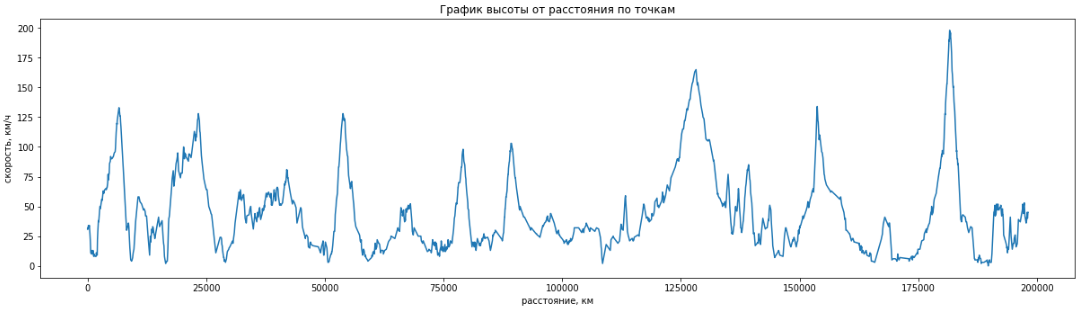
\includegraphics[scale = 0.6]{График по точкам.png}

Далее получаем из этого массива кубический интеполянт и сравниваем его с предыдущим графиком:

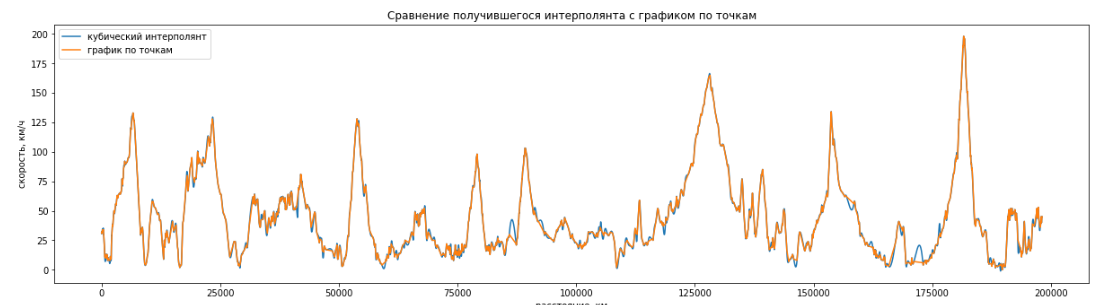
\includegraphics[scale = 0.6]{Сравнение графиков.png}

\subsection*{Запись уравнения движения ТС}
\subsubsection*{Уравнение при P=const}
На ТС на треки действуют:
\begin{itemize}
    \item Сила тяжести
    \item Сила движения (трение колёс, которое и приводит ТС в движение)
    \item Сила трения качения 
    \item Сила сопротивления воздуха
    \item Сила реакции опоры
\end{itemize}

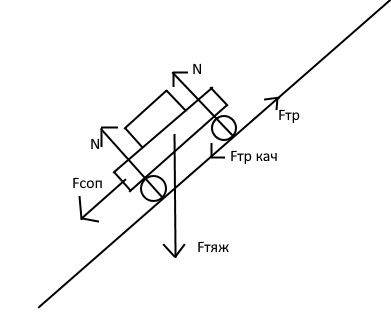
\includegraphics{Зарисовка.png}

 Нам также понадобится плотность воздуха для вычисления его сопротивления ($\rho$). Выгружаем данные с \href{https://ru.wikipedia.org/wiki/Плотность_воздуха}{сайта} в формате BeautifulSoup и парсим, получая переменную с таблицей плотности воздуха от температуры, затем с помощью цикла находим нужную температуру и плотность воздуха и используем её. Для определения угла $\alpha$, мы поместим переменную alpha\_x в которой будет хранится производная от интерполянта на любой точке трека.
 
 Запишем ОДУ второго порядка движения ТС, мы будем считать начальную скорость $v\rightarrow0$:
 \[
 x = x_0 + x't + \dfrac{x"t^2}{2}
 \]
где 
\[
x'' = \dfrac{F}{m} =  \dfrac{(\frac{P}{v_0}-mg\sin{\alpha} - \frac{f}{R}mg\cos{\alpha} - C_x\frac{\rho v_0^2}{2}S)t^2}{2m}
\]

С помощью замены $x'=v_0$ и $v' = \dfrac{(\frac{P}{v_0}-mg\sin{\alpha} - \frac{f}{R}mg\cos{\alpha} - C_x\frac{\rho v_0^2}{2}S)t^2}{2m}$ мы можем привести это уравнение к системе уравнений первого порядка:
\[
\begin{cases}
x' = v_0\\
v'=\dfrac{(\frac{P}{v_0}-mg\sin{\alpha} - \frac{f}{R}mg\cos{\alpha} - C_x\frac{\rho v_0^2}{2}S)t^2}{2m}
\end{cases}
\]
Посмотрим зависимость силы двигателя от скорости автомобиля:
\begin{figure}[h!]
    \centering
    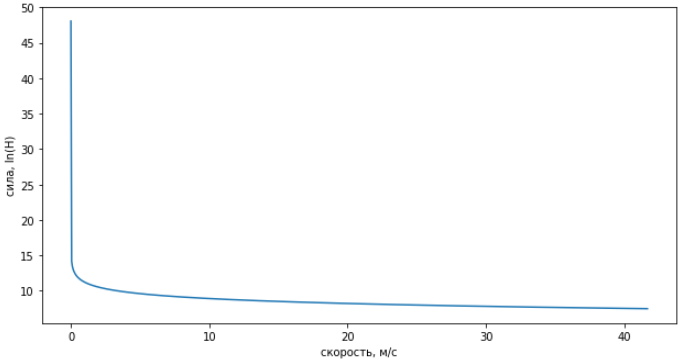
\includegraphics[scale = 0.6]{Скорость_сила.png}
    \caption{зависимость силы от скорости ТС}
\end{figure}

Как можно увидеть сила двигателя всегда положительна, но в реальных условиях водитель ограничен максимальной скоростью на пути, но даже если сила двигателя будет 0, то может возникнуть ситуация, где водитель катиться со склона и скорость не будет уменьшаться.
\subsubsection*{Уравнение при динамической мощности}
Добавим к движущей силе (Fтр) коффициент $1-\frac{3.6v_0}{100}$, который показывает изменения мощности двигателя, в зависимости от текущей скорости к максимальной на треке (100~км/ч = (100 * 1000/3600)~м/с = $\frac{100}{3.6}$~м/с). Посмотрим как коэффициент повлиял на зависимость силы от скорости:
\begin{figure}[h!]
    \centering
    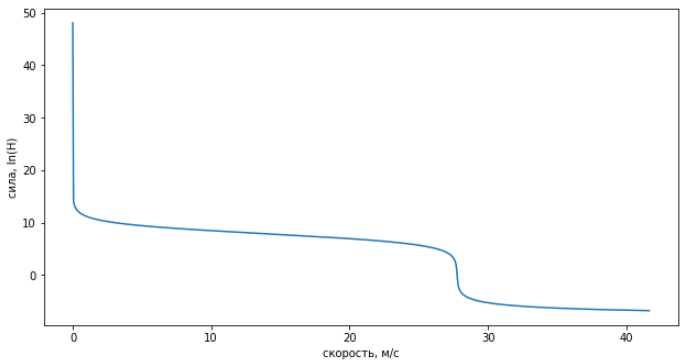
\includegraphics[scale = 0.6]{Скорость_сила_коэф.png}
    \caption{зависимость силы от скорости ТС при динамической мощности}
\end{figure}

Как видно сила может становиться отрицательной, эту силу мы можем считать торможением двигателя, т.е. переход ТС на первую передачу для машин с двигателем внутреннего сгорания, для электрокаров это отключение двигателя и перевода механической энергии в элетрическую.

Новая система уравнений будет выглядеть так:

\[
\begin{cases}
x' = v_0\\
v' = \dfrac{(\frac{P}{v_0}(1-\dfrac{3.6v_0}{100})-mg\sin{\alpha} - \frac{f}{R}mg\cos{\alpha} - C_x\frac{\rho v_0^2}{2}S)t^2}{2m}
\end{cases}
\]
\subsection*{Расчёт векторов состояния}
Напишем функцию, возвращающую полученную систему уравнений в виде вектора состояния (x,v), где x - пройденное ТС расстояние и v - скорость в тот момент.

Далее напишем функцию останова (solout) для интегрирования, которая возвращает 0, если можно продолжать интегрирование и -1, если нельзя, также она будет добавлять вектор состояния в массив, а также момент времемни и коэффициент мощности двигателя.

При помощи scipy.integrate.ode и функции останова интегрируем функцию движения ТС, в результате получаем массив со всеми векторами состояния, моментами времени и коэффициентами мощости.
\newpage
\subsection*{Некоторые расчёты с помощью массива векторов состояния}
Скорости:
\begin{itemize}
    \item минимальная скорости в пути - 46~км/ч (поиск минимальной скорости идёт спустя 10 минут после старта)
    \item средняя скорость в пути - 74~км/ч 
    \item максимальная скорость в пути - 104~км/ч
\end{itemize}

Также рассчитаем кол-во бензина затраченное на преодоления пути. Для этого найдём совершённую ТС работу, умножая мощность на коэффициент и на разность времени между двумя соседними точками и сложим получившиеся работы, далее делим результат на КПД двигателя внутреннего сгорания (0.4) и переводим в литры, поделив на 10~кВт*ч/л. Результат - 15.9~л
\newpage
\subsection*{Графики}

\begin{figure}[h!]
    \centering
    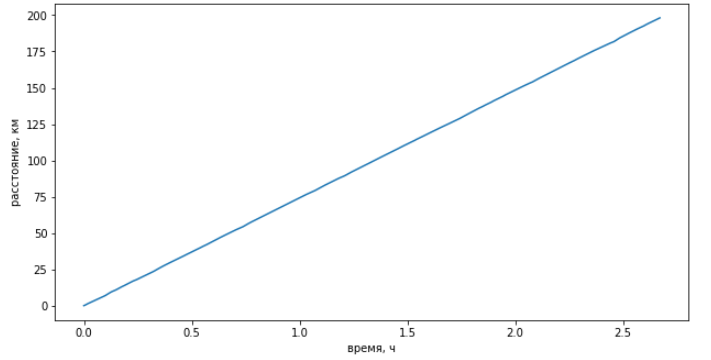
\includegraphics[scale = 0.6]{Расстояние_время.png}
    \caption{Расстояние от времени ТС}
\end{figure}

 Как видим расстояние имеет практические линейную зависимости от времени.
 
 \begin{figure}[h!]
     \centering
     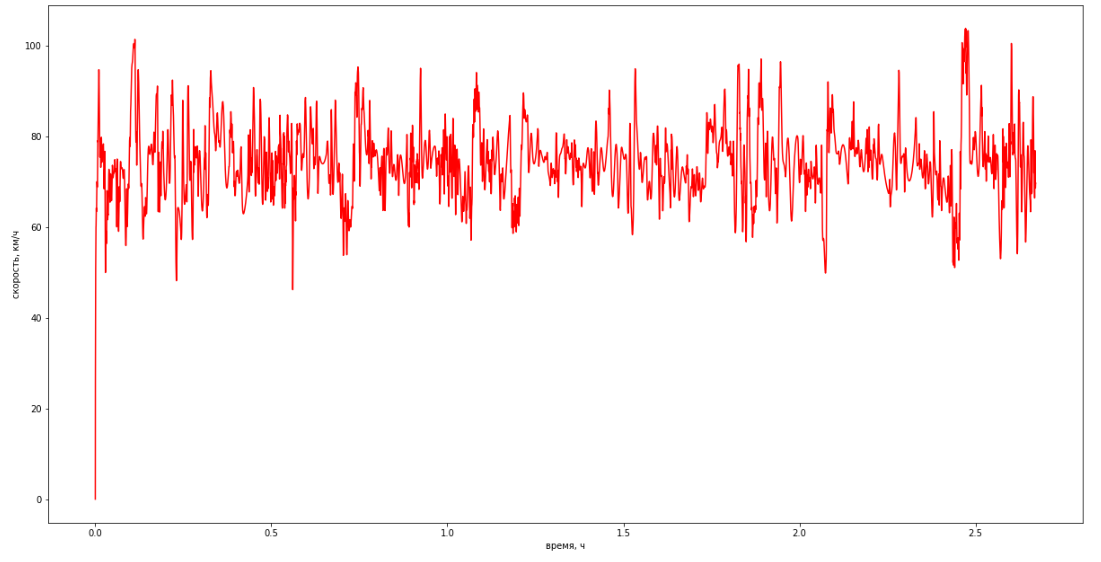
\includegraphics[scale =0.55]{скорость_время.png}
     \caption{Скорость от времени}
 \end{figure}
 
 \begin{figure}[h!]
     \centering
     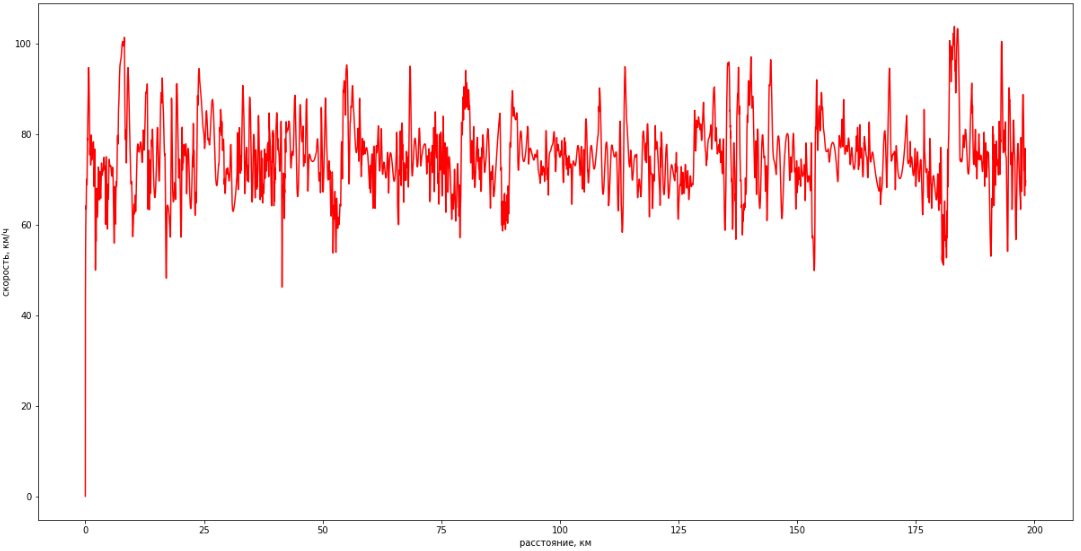
\includegraphics[scale = 0.55]{Скорость_расстояние.png}
     \caption{Скорость от расстояния}
 \end{figure}
 
 Графики скорость от времени и расстояния являются практически идентичными, что ещё раз показывает их линейную зависимость.
 
 \begin{figure}[h!]
     \centering
     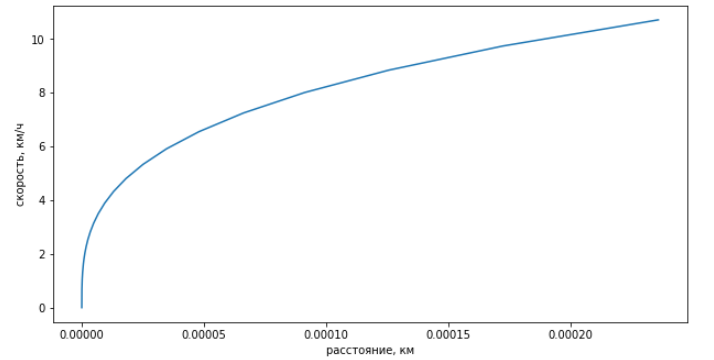
\includegraphics[scale = 0.95]{Скорость10.png}
     \caption{График расстояния от скорости, где скорость была меньше 10~км/ч}
 \end{figure}
 
 \begin{figure}[h!]
     \centering
     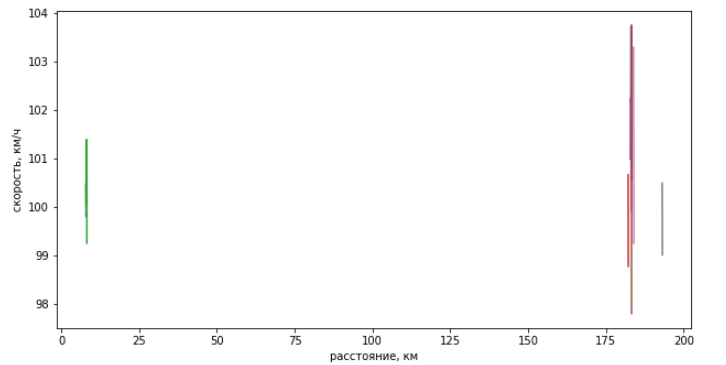
\includegraphics[scale = 0.8]{скорость100.png}
     \caption{График скорости от расстояния, где ТС движется более чем 100~км/ч}
 \end{figure}
 
 При достижении 100~км/ч ТС быстро сбрасывает скорость, в виду отрицательного ускорения (в реальности можно предположить, что водитель перешёл на первую передачу)
 
 Проверим это, приблизив первый участок превышения скорости
 \begin{figure}[h!]
     \centering
     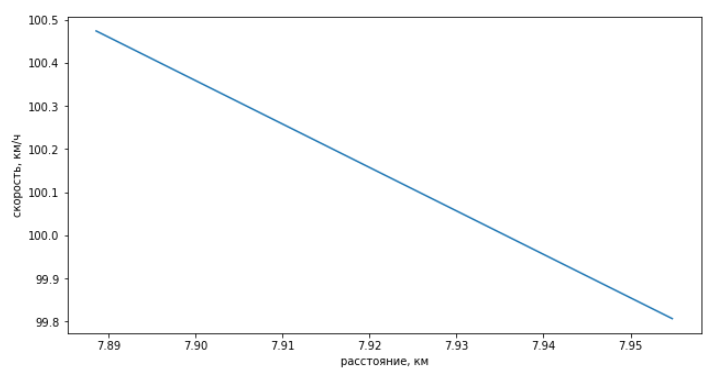
\includegraphics[scale = 0.7]{Скорость100один.png}
     \caption{Первый участок, где ТС превысил скорость}
 \end{figure}
 
  \begin{figure}[h!]
     \centering
     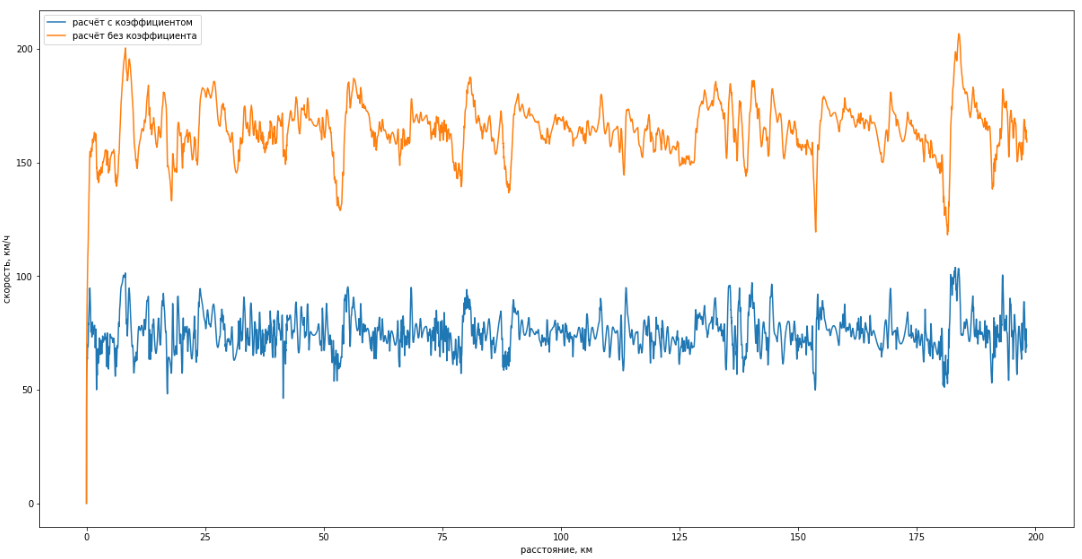
\includegraphics[scale = 0.55]{Сравнение_скорости.png}
     \caption{Первый участок, где ТС превысил скорость}
 \end{figure}
 
 Из этого графика мы видим, как отличается скорость ТС без коэффициента, от чего такая модель имела бы сильную погрешность и её было бы сложно наложить на реальность, если максимальная скорость меньше 200~км/ч.
 \newpage
 \section*{Заключение}
 
 Мы получили программу, способную рассчитать приблизительное движение ТС по треку и получили данные о его состоянии на протяжении всего пути, что позволяет использовать программу для организации маршрута и возможность выбора оптимального транспорта путём изменения характеристик ТС и сравнением результатов. Также есть возможность доработать уравнение движения для получения более точных данных а также использовать полученные векторы состояния для расчёта другой информации, если это необходимо.
 \newpage
 \begin{thebibliography}{9}
 \bibitem{resist}Онищенко О. Г., Коробко Б. А., Ващенко К. М. Структура, кинематика и динамика механизмов //Полтава: ПолНТУ. – 2010.
 \bibitem{air}Юрьев Б. Н. Экспериментальная аэродинамика. – Рипол Классик, 2013.
 \bibitem{ode}Ильина В. А., Силаев П. К. Численные методы для физиков-теоретиков. – Институт компьютерных исследований, 2004. – С. 118-118.
 \bibitem{NumpyScipy}Bressert E. SciPy and NumPy: an overview for developers. – " O'Reilly Media, Inc.", 2012.
 \bibitem{matplotlib}Tosi S. Matplotlib for Python developers. – Packt Publishing Ltd, 2009.
 \bibitem{RequestsBS4}Mitchell R. Web scraping with Python: Collecting more data from the modern web. – " O'Reilly Media, Inc.", 2018.
 \bibitem{Pandas}McKinney W. et al. pandas: a foundational Python library for data analysis and statistics //Python for High Performance and Scientific Computing. – 2011. – Т. 14. – №. 9.
 \end{thebibliography}
 
 \newpage
 \section*{Приложение}

 
\noindent import numpy as np\\
import requests\\
import pandas as pd\\
from bs4 import BeautifulSoup\\
import math\\
import matplotlib.pyplot as plt\\
import scipy.interpolate\\
import scipy.integrate\\

\noindent def dist(llat1,llong1,llat2,llong2):

    rad = 6372795
    lat1 = llat1*math.pi/180.
    
    lat2 = llat2*math.pi/180.
    
    long1 = llong1*math.pi/180.
    
    long2 = llong2*math.pi/180.
    
    cl1 = math.cos(lat1)
    
    cl2 = math.cos(lat2)
    
    sl1 = math.sin(lat1)
    
    sl2 = math.sin(lat2)
    
    delta = long2 - long1
    
    cdelta = math.cos(delta)
    
    sdelta = math.sin(delta)
    
    y = math.sqrt(math.pow(cl2*sdelta,2)+math.pow(cl1*sl2-sl1*cl2*cdelta,2))
    
    x = sl1*sl2+cl1*cl2*cdelta
    
    ad = math.atan2(y,x)
    
    dist = ad*rad
    
    return (dist)
    
    \noindent data  = np.genfromtxt('Vladivostok-Nahodka.csv',dtype=float,delimiter=',')
    
    \noindent data = data[1:]

    \noindent route = [[0,data[0][2]]]
    
    \noindent for i in range(len(data)-1):
    
    a = [dist(data[i][0],data[i][1],data[i+1][0],data[i+1][1]),data[i+1][2]]
    
    route.append(a)
    
    \noindent route=np.array(route)
    
    \noindent route[:,0]=np.cumsum(route[:,0],dtype=float)
    
    \noindent \% matplotlib inline
    
    \noindent xs = np.linspace(0,route[len(route)-1,0],1000000)
    
    \noindent h\_x = scipy.interpolate.InterpolatedUnivariateSpline(route[:,0],route[:,1], k=3)
    
    \noindent fg = plt.figure(figsize=(20, 5), constrained\_layout=True)
    
    \noindent axes = fg.add\_axes([0.1, 0.1, 0.8, 0.8])
    
    \noindent plt.plot(route[:,0],route[:,1])
    
    \noindent axes.set\_xlabel('расстояние, м')
    
    \noindent axes.set\_ylabel('высота, м')
    
    \noindent axes.set\_title('График высоты от расстояния по точкам')
    
    \noindent fg = plt.figure(figsize=(20, 5), constrained\_layout=True)
    
    \noindent xs = np.linspace(0,route[len(route)-1,0],1000000)
    
    \noindent axes = fg.add\_axes([0.1, 0.1, 0.8, 0.8])
    
    \noindent plt.plot(xs,h\_x(xs),label = 'кубический интерполянт')
    
    \noindent plt.plot(route[:,0],route[:,1],label = 'график по точкам')
    
    \noindent axes.legend(loc=2);
    
    \noindent axes.set\_title('Сравнение получившегося интерполянта с графиком по точкам')
    
    \noindent axes.set\_xlabel('расстояние, м')
    
    \noindent axes.set\_ylabel('высота, м')
    
    \noindent fg = plt.figure(figsize=(20, 5), constrained\_layout=True)
     
    \noindent xs = np.linspace(0,route[len(route)-1,0],1000000)
     
    \noindent axes = fg.add\_axes([0.1, 0.1, 0.8, 0.8])
    
    \noindent plt.plot(xs,h\_x(xs))
     
    \noindent axes.set\_xlabel('расстояние, м')
     
    \noindent axes.set\_ylabel('высота, м')
     
    \noindent alpha\_x = h\_x.derivative(n=1)
    
    \noindent dens\_url = "https://ru.wikipedia.org/wiki/Плотность\_воздуха"
    
    \noindent wiki\_req = requests.get(dens\_url).text
    
    \noindent density = BeautifulSoup(wiki\_req,'lxml')
    
    \noindent density = density.find('table',class\_='wikitable')

    \noindent a=density.find\_all('td')

    \noindent table = []
    
    \noindent for field in a:
    
    table.append(str(field))
    
    \noindent for i in range(len(table)):
    
    table[i] = table[i].replace('<td>','''')
    
    table[i] = table[i].replace('</td>','''')
    
    table[i] = table[i].replace('$\backslash$n','''')
    
    table[i] = table[i].replace(',','.')
    
    table[i] = table[i].replace(',','.')
    
    table[i] = table[i].replace('--','-') 
    
    \noindent for i in range(len(table)//4):
    
    table[i*4] = int(table[i*4])
    
    table[i*4+2] = float(table[i*4+2])
    
\noindent m = 1500

\noindent S = 2.5

\noindent Cx= 0.25

\noindent P = 735.5*125

\noindent kp= 0.8

\noindent kr = 0.05

\noindent t = -10

\noindent for i in range(len(table)//4):

    if(table[i*4]==t):
    
    \ \ \ \ ro = table[i*4+2]
    
    \noindent def motion\_ode(t,s,alpha\_x,S,kp,m,kr,Cx,ro,P):
    
    alpha = math.atan(alpha\_x(s[0]))
    
    g=9.81
    
    gx=g*math.sin(alpha)
    
    gy=g*math.cos(alpha)
    


    F = (P*kp)/(s[1]*m)
    
    k=(1-s[1]*3.6/100)
    
    return [s[1],F*k - gx - kr * gy - (Cx*ro*s[1]*s[1]*S)/(2*m)]

\noindent fig = plt.figure(figsize=(10, 5), constrained\_layout=True)

\noindent axes = fig.add\_axes([0.1, 0.1, 0.8, 0.8])

\noindent varr=np.linspace(1e-16,150/3.6,800)

\noindent Farr=[]

\noindent for v in varr:

    acc = (P*kp)/(v)

    if(acc > 0 ):
    
    \ \ \ \ Farr.append(math.log(acc))
        
    elif(acc < 0):
    
    \ \ \ \ Farr.append(-math.log(abs(acc)))
        
    else:
    
    \ \ \ \ Farr.append(0)
        
\noindent axes.plot(varr,Farr)

\noindent axes.set\_xlabel('скорость, м/с')

\noindent axes.set\_ylabel('сила, ln(Н)')

\noindent fig = plt.figure(figsize=(10, 5), constrained\_layout=True)

\noindent axes = fig.add\_axes([0.1, 0.1, 0.8, 0.8])

\noindent Farr=[]

\noindent for v in varr:

    acc = (1-v*3.6/100)*(P*kp)/(v)

    if(acc > 0 ):
    
    \ \ \ \ Farr.append(math.log(acc))
        
    elif(acc < 0):
    
    \ \ \ \ Farr.append(-math.log(abs(acc)))
        
    else:
    
    \ \ \ \ Farr.append(0)
        
\noindent axes.plot(varr,Farr)

\noindent axes.set\_xlabel('скорость, м/с')

\noindent axes.set\_ylabel('сила, ln(Н)')


\noindent def stopLength(t,s,L,lst):

    k=1-s[1]*3.6/100
    
    lst.append(np.hstack((s,t,k)))
    
    if (s[0] >= L):
    
    \ \ \ \ return -1
        
    return 0 
    
\noindent L=route[-1,0]

\noindent v0 = 1e-16

\noindent s0 = (0,v0)

\noindent prop = scipy.integrate.ode(lambda t, s: motion\_ode(t,s,alpha\_x,S,kp,m,kr,Cx,ro,P))

\noindent prop.set\_initial\_value(s0, 0)

\noindent prop.set\_integrator('dopri5', nsteps=1e5)

\noindent lst = []

\noindent prop.set\_solout(lambda t, s: stopLength(t, s, L, lst))

\noindent prop.integrate(1e10)

\noindent arr = np.asarray(lst)

\noindent arr[:,0] = arr[:,0] / 1000

\noindent arr[:,1]=arr[:,1] * 3.6

\noindent arr[:,2]=arr[:,2] / 3600

\noindent fig = plt.figure(figsize=(10, 5), constrained\_layout=True)

\noindent axes = fig.add\_axes([0.1, 0.1, 0.8, 0.8])

\noindent axes.plot(arr[:,2],arr[:,0])

\noindent axes.set\_xlabel('время, ч')

\noindent axes.set\_ylabel('расстояние, км')

\noindent fig = plt.figure(figsize=(20, 10), constrained\_layout=True)

\noindent axes = fig.add\_axes([0.1, 0.1, 0.8, 0.8])

\noindent axes.plot(arr[:,2],arr[:,1],'r')

\noindent axes.set\_xlabel('время, ч')

\noindent axes.set\_ylabel('скорость, км/ч')

\noindent fig = plt.figure(figsize=(20, 10), constrained\_layout=True)

\noindent axes = fig.add\_axes([0.1, 0.1, 0.8, 0.8])

\noindent axes.plot(arr[:,0],arr[:,1],'r')

\noindent axes.set\_xlabel('расстояние, км')

\noindent axes.set\_ylabel('скорость, км/ч')

\noindent flag = False

\noindent vmax = arr[0,1]

\noindent for row in arr[1:]:

    if(row[2]>0.25 and flag == False):
    
    \ \ \ \ vmin = row[1]
        
    \ \ \ \ flag = True
        
    if (flag and vmin>row[1]):
    
    \ \ \ \ vmin = row[1]
        
    if(vmax<row[1]):
    
    \ \ \ \ vmax = row[1]
        
\noindent print("средняя скорость -", round(arr[-1,0]/arr[-1,2],1))

\noindent print("максимальная скорость -",round(vmax,1))

\noindent print(" минимальная скорость -",round(vmin,1))

\noindent A=0

\noindent for i in range(len(arr)-1):

    deltaT=(arr[i+1,2]-arr[i,2])
    
    A+=P*arr[i,3]*deltaT*3600/0.4
    
\noindent litres = A/36000000

\noindent print('Кол-во литров для преодоления пути -',round(litres,1))

\noindent fig = plt.figure(figsize=(10, 5), constrained\_layout=True)

\noindent flag = False

\noindent start, end = 0,0

\noindent axes = fig.add\_axes([0.1, 0.1, 0.8, 0.8])

\noindent for i in range(len(arr)):

    if(arr[i,1]<10 and flag == False):
    
    \ \ \ \ start = i
        
    \ \ \ \ flag = True
        
    if(arr[i,1]>=10 and flag == True):
    
    \ \ \ \ end=i+1
        
    \ \ \ \ flag = False
        
    if(end>0):
    
    \ \ \ \ axes.plot(arr[start:end,0],arr[start:end,1])
        
    \ \ \ \ start = 0
        
    \ \ \ \ end = 0

\noindent axes.set\_xlabel('расстояние, км')

\noindent axes.set\_ylabel('скорость, км/ч')

\noindent fig = plt.figure(figsize=(10, 5), constrained\_layout=True)

\noindent flag = False

\noindent start, end = 0,0

\noindent axes = fig.add\_axes([0.1, 0.1, 0.8, 0.8])

\noindent for i in range(len(arr)):

    if(arr[i,1]>100 and flag == False):
    
    \ \ \ \ start = i
        
    \ \ \ \ flag = True
        
    if(arr[i,1]<=100 and flag == True):
    
    \ \ \ \ end=i+1
        
    \ \ \ \ flag = False
        
    if(end>0):
    
    \ \ \ \ plt.plot(arr[start:end,0],arr[start:end,1])
        
    \ \ \ \ start = 0
        
    \ \ \ \ end = 0
        
\noindent axes.set\_xlabel('расстояние, км')

\noindent axes.set\_ylabel('скорость, км/ч')

\noindent fig = plt.figure(figsize=(10, 5), constrained\_layout=True)

\noindent axes = fig.add\_axes([0.1, 0.1, 0.8, 0.8])

\noindent flag = False

\noindent start, end = 0,0

\noindent for i in range(len(arr)):

    if(arr[i,1]>100 and flag == False):
    
    \ \ \ \ start = i
    
    \ \ \ \ flag = True
    
    if(arr[i,1]<=100 and flag == True):
    \ \ \ \ end=i+1
    
    \ \ \ \ flag = False
    
    if(end>0):
    
    \ \ \ \ plt.plot(arr[start:end,0],arr[start:end,1])
    
    \ \ \ \ start = 0
    
    \ \ \ \ end = 0
    
    \ \ \ \ break
    
\noindent axes.set\_xlabel('расстояние, км')

\noindent axes.set\_ylabel('скорость, км/ч')

\noindent fig = plt.figure(figsize=(20, 10), constrained\_layout=True)

\noindent axes = fig.add\_axes([0.1, 0.1, 0.8, 0.8])

\noindent axes.plot(arr[:,0],arr[:,1],label = 'расчёт с коэффициентом')

\noindent axes.plot(arr2[:,0],arr2[:,1],label = 'расчёт без коэффициента')

\noindent axes.legend(loc=2);

\noindent axes.set\_xlabel('расстояние, км')

\noindent axes.set\_ylabel('скорость, км/ч')

\end{document}
